\documentclass[conference]{IEEEtran}
\IEEEoverridecommandlockouts
\usepackage{cite}
\usepackage{amsmath,amssymb,amsfonts}
\usepackage{graphicx}
\usepackage{textcomp}
\usepackage{xcolor}
\usepackage{url}

\newcommand{\ket}[1]{\left|#1\right\rangle}
\newcommand{\bra}[1]{\left\langle#1\right|}
\newcommand{\avg}[1]{\left\langle#1\right\rangle}

\begin{document}

\title{Simulating Spin Dephasing from Measured Magnetic Field Noise:\\
Ramsey, Hahn Echo and CPMG Dynamical Decoupling}

\author{\IEEEauthorblockN{1\textsuperscript{st} Marcin Lubonski}
\IEEEauthorblockA{\textit{School of Electrical Engineering and Telecommunications} \\
\textit{University of NSW, Sydney, Australia} \\
email: marcin.lubonski@gmail.com}
}

\maketitle

\begin{abstract}
We simulate the dephasing of an ensemble of one hundred spin qubits driven by
experimentally recorded traces of effective magnetic field noise. Each trace is
treated as the noise realisation experienced by one spin, and the qubit state is
propagated as a density matrix through explicit instantaneous rotation operators
and free evolution governed by the accumulated stochastic phase. The noise power
spectral density is estimated by two independent routes, Welch periodogram
averaging over the ensemble and the Fourier transform of the ensemble averaged
autocorrelation function, and is found to follow an inverse square frequency law
across the accessible band, consistent with a Lorentzian spectrum whose knee lies
below the inverse record length. Coherence decay curves are computed for a free
induction Ramsey sequence, a Hahn echo, and Carr Purcell Meiboom Gill sequences
with two, four and eight refocusing pulses. Fitting a stretched exponential to
each curve yields a free induction dephasing time of seventy one microseconds
with a near Gaussian exponent, rising to four point four milliseconds under eight
pulse decoupling. Coherence times predicted from the measured spectrum through
the filter function formalism agree with the trace based simulation to within ten
percent with no adjustable parameters, and the extracted decoupling gain follows a
two thirds power law in pulse number as expected for Lorentzian noise.
\end{abstract}

\begin{IEEEkeywords}
spin qubit, decoherence, dephasing, density matrix, dynamical decoupling, Hahn
echo, CPMG, power spectral density, filter function
\end{IEEEkeywords}

\section{Introduction}

The practical utility of a spin qubit is bounded by the time over which it
retains a well defined quantum phase. Isolated quantum systems evolve unitarily
and reversibly, but a real spin is embedded in an environment whose fluctuating
degrees of freedom imprint a random phase on the qubit. When these fluctuations
couple to the spin as an effective magnetic field along the quantisation axis,
the resulting loss of phase information is called dephasing, and it is typically
the dominant error channel in solid state spin qubits.

Two questions follow. First, given a measured record of the environmental noise,
can one predict quantitatively how fast coherence will decay? Second, how much of
that decay can be recovered by pulse sequences that refocus the accumulated
phase? This paper addresses both using an ensemble of one hundred recorded noise
traces. Section~\ref{sec:theory} develops the theory: unitary evolution under the
Schr\"odinger equation, the density matrix description of a mixed ensemble, and
the pulse sequences used to suppress dephasing. Section~\ref{sec:psd} describes
the estimation of the noise power spectral density and the filter function
formalism that links it to coherence decay. Section~\ref{sec:methods} sets out
the numerical implementation, Section~\ref{sec:results} presents the simulated
decay curves and extracted coherence times, and Section~\ref{sec:discussion}
interprets the results.

\section{Theory}\label{sec:theory}

\subsection{Unitary evolution}

The state $\ket{\psi(t)}$ of a closed quantum system obeys the time dependent
Schr\"odinger equation
\begin{equation}
i\hbar\,\frac{\partial}{\partial t}\ket{\psi(t)} = \hat{H}\ket{\psi(t)},
\label{eq:tdse}
\end{equation}
where $\hat{H}$ is the Hamiltonian. For a time independent Hamiltonian the
solution is generated by the unitary propagator
\begin{equation}
\ket{\psi(t)} = \hat{U}(t)\ket{\psi(0)}, \qquad
\hat{U}(t) = e^{-i\hat{H}t/\hbar}.
\label{eq:propagator}
\end{equation}
For a spin one half in a magnetic field $\mathbf{B}$ the interaction is the
Zeeman coupling $\hat{H} = -\gamma\,\mathbf{B}\cdot\hat{\mathbf{S}}$, with
$\gamma$ the gyromagnetic ratio and $\hat{\mathbf{S}} = (\hbar/2)\boldsymbol{\sigma}$
the spin operator. A field along $z$ therefore produces the Hamiltonian
$\hat{H}_0 = -\gamma B_z \hat{S}_z$ and a precession of the transverse spin
components at the Larmor frequency $\omega_0 = \gamma B_z$.

Equation~\eqref{eq:propagator} describes perfect, reversible evolution. It cannot
by itself describe decoherence, because a unitary map preserves the purity
$\mathrm{Tr}(\rho^2)$ of a state. Decoherence arises when the system is coupled to
an environment whose state is not tracked.

\subsection{Density matrix and coherence}

An ensemble of spins in states $\ket{\psi_i}$ with probabilities $p_i$ is
described by the density matrix
\begin{equation}
\rho = \sum_i p_i \ket{\psi_i}\bra{\psi_i},
\end{equation}
which evolves under the von Neumann equation
$\dot{\rho} = -\tfrac{i}{\hbar}[\hat{H},\rho]$ for unitary dynamics, and under the
Lindblad master equation
\begin{equation}
\frac{d\rho}{dt} = -\frac{i}{\hbar}\left[\hat{H},\rho\right] + \mathcal{L}(\rho)
\label{eq:lindblad}
\end{equation}
when the environment is traced out, the superoperator $\mathcal{L}$ carrying the
dissipative and dephasing terms. In the basis $\{\ket{0},\ket{1}\}$ the diagonal
elements $\rho_{00}$ and $\rho_{11}$ are the populations, while the off diagonal
element $\rho_{01}$ is the coherence, encoding the definiteness of the relative
phase. Pure dephasing is the decay of $\rho_{01}$ at fixed populations.

The present work does not postulate a Lindblad operator. Instead, since the noise
record is available explicitly, each spin is evolved unitarily under its own
realisation of the field and the ensemble average is taken at the end. This is
exact for classical noise and does not require the Markov approximation implicit
in~\eqref{eq:lindblad}; the irreversible looking decay emerges from averaging over
realisations rather than being imposed.

\subsection{Stochastic phase accumulation}

Let spin $i$ experience the fluctuating field $B_i(t)$ along $z$, so that
\begin{equation}
\hat{H}_i(t) = -\gamma B_i(t)\,\hat{S}_z
= -\frac{\hbar}{2}\,\gamma B_i(t)\,\sigma_z .
\end{equation}
Because $\hat{H}_i(t)$ commutes with itself at different times, the propagator is
obtained without time ordering,
\begin{equation}
\hat{U}_i(t) = \exp\left[-\frac{i}{2}\phi_i(t)\,\sigma_z\right], \quad
\phi_i(t) = \gamma\!\int_0^t\! B_i(t')\,dt' .
\label{eq:phase}
\end{equation}
The random variable $\phi_i$ is the accumulated phase. Starting from the
superposition $\ket{+}=(\ket{0}+\ket{1})/\sqrt{2}$, the coherence of spin $i$
acquires the factor $e^{-i\phi_i}$, and the ensemble averaged coherence is
\begin{equation}
W(\tau) \equiv 2\left|\avg{\rho_{01}}\right| = \left|\avg{e^{-i\phi}}\right| .
\label{eq:W}
\end{equation}
No individual spin loses coherence; it is the spread of $\phi$ across the
ensemble that suppresses the average. For zero mean Gaussian noise the average
can be evaluated in closed form,
\begin{equation}
W(\tau) = \exp\left[-\tfrac{1}{2}\avg{\phi^2(\tau)}\right] \equiv e^{-\chi(\tau)} ,
\label{eq:gaussian}
\end{equation}
which defines the decoherence function $\chi$.

Two limits are instructive. If the noise is effectively static over the
measurement, $\phi = \gamma B \tau$ with $B$ drawn from a distribution of width
$\sigma_B$, giving a Gaussian decay
\begin{equation}
W(\tau) = \exp\left[-\tfrac{1}{2}\gamma^2\sigma_B^2\tau^2\right], \qquad
T_2^{*} = \frac{\sqrt{2}}{\gamma\sigma_B},
\label{eq:quasistatic}
\end{equation}
where $T_2^*$ is defined by $W(T_2^*)=e^{-1}$. If instead the noise is
delta correlated, $\avg{\phi^2}$ grows linearly in $\tau$ and the decay is a
simple exponential. The exponent $p$ in the stretched exponential
$W=\exp[-(\tau/T_2)^p]$ therefore diagnoses the noise correlation time.

\subsection{Pulse sequences}\label{sec:sequences}

\begin{figure}[t]
\centerline{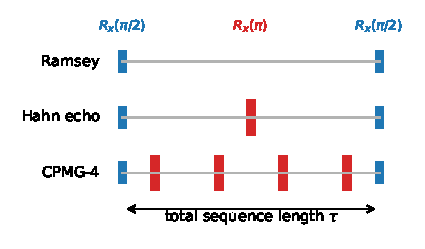
\includegraphics[width=\columnwidth]{fig_sequences.pdf}}
\caption{Pulse sequences studied. Narrow bars are $\pi/2$ pulses about $x$, wide
bars are $\pi$ refocusing pulses. All pulses are instantaneous and the abscissa is
the total sequence length $\tau$.}
\label{fig:sequences}
\end{figure}

All sequences considered here begin by rotating the ground state $\ket{0}$ onto
the equator of the Bloch sphere with the instantaneous rotation
\begin{equation}
R_x(\theta) = \exp\left[-\frac{i\theta}{2}\sigma_x\right]
= \cos\frac{\theta}{2}\,\mathbb{1} - i\sin\frac{\theta}{2}\,\sigma_x ,
\end{equation}
taking $\theta = \pi/2$. They differ in the refocusing pulses applied during the
subsequent evolution, as sketched in Fig.~\ref{fig:sequences}.

\emph{Ramsey.} The spin evolves freely for the whole interval $\tau$ and the
phase~\eqref{eq:phase} accumulates without interruption. All noise frequencies
down to zero contribute, so the static spread of the field is fully sampled and
the decay time is the inhomogeneous dephasing time $T_2^{*}$. A second $\pi/2$
pulse converts the surviving coherence into a population difference for readout.

\emph{Hahn echo.} A single $\pi$ pulse at $\tau/2$ inverts the spin, so the phase
accumulated in the second half enters with the opposite sign. The net phase
becomes
\begin{equation}
\phi = \gamma\left[\int_0^{\tau/2}\! B\,dt' - \int_{\tau/2}^{\tau}\! B\,dt'\right],
\end{equation}
which vanishes identically for a static field. The echo therefore removes the
quasi static contribution and the resulting decay time is the intrinsic $T_2$.

\emph{CPMG.} Extending the idea, $N$ refocusing pulses are placed at
\begin{equation}
t_j = \frac{(2j-1)\tau}{2N}, \qquad j=1,\dots,N ,
\end{equation}
the Carr Purcell Meiboom Gill timing; the Hahn echo is the case $N=1$. Each
additional pulse shortens the interval over which phase accrues coherently, so
the sequence becomes progressively blind to low frequency noise. Because the pulses
are applied about the same axis as the initial rotation, CPMG is also robust
against small pulse amplitude errors, although this is immaterial here since all
pulses are taken to be ideal and instantaneous.

\section{Noise Spectrum and Filter Functions}\label{sec:psd}

\subsection{Spectral estimation}

The noise is assumed stationary and ergodic, so ensemble and time averages
coincide and the autocorrelation function
\begin{equation}
R_B(s) = \avg{B(t)B(t+s)}
\end{equation}
depends only on the lag $s$. The Wiener Khinchin theorem relates it to the
one sided power spectral density,
\begin{equation}
S_B(f) = 2\int_{-\infty}^{\infty} R_B(s)\,e^{-i2\pi f s}\,ds , \qquad f \ge 0 ,
\label{eq:wk}
\end{equation}
normalised so that $\sigma_B^2 = \int_0^\infty S_B(f)\,df$.

Two estimators are used. The first evaluates~\eqref{eq:wk} directly: the
autocorrelation of each trace is computed by fast Fourier transform, averaged over
the ensemble, tapered with a Hann lag window to suppress the poorly determined
long lag estimates, and transformed. The second is Welch's method, applied to each
trace over its full length with a Hann data window and then averaged across the
one hundred traces; ergodicity makes this ensemble average a legitimate substitute
for the segment averaging normally used to reduce periodogram variance, at no cost
in frequency resolution.

\subsection{From spectrum to coherence}

For Gaussian noise the decoherence function in~\eqref{eq:gaussian} can be written
as an overlap between the noise spectrum and a filter determined entirely by the
pulse timing,
\begin{equation}
\chi(\tau) = \frac{1}{2\pi}\int_0^\infty
S_\omega(\omega)\,\left|\tilde{f}(\omega,\tau)\right|^2 d\omega ,
\label{eq:chi}
\end{equation}
where $S_\omega(\omega) = \gamma^2 S_B(\omega/2\pi)/4\pi$ is the angular frequency
spectrum of the phase noise and
\begin{equation}
\tilde{f}(\omega,\tau) = \int_0^{\tau} y(t)\,e^{i\omega t}\,dt
\label{eq:filter}
\end{equation}
is the Fourier transform of the toggling function $y(t)=\pm 1$, which switches
sign at each $\pi$ pulse. Equation~\eqref{eq:chi} makes the role of the sequences
transparent: Ramsey has $y=+1$ throughout, so $|\tilde{f}|^2$ peaks at
$\omega=0$ and the sequence is maximally sensitive to slow noise; each refocusing
pulse pushes the passband up to $\omega \approx \pi N/\tau$, where a decreasing
spectrum supplies less power. Because $\tilde{f}$ is piecewise analytic, the
integral in~\eqref{eq:filter} reduces to a sum over pulse edges and is evaluated
without further approximation.

\section{Numerical Method}\label{sec:methods}

The data consist of one hundred traces of effective field noise sampled at
$\Delta t = 2.5\;\mu$s for $7603$ points, a record length of $19.01$~ms per trace.
The gyromagnetic ratio is taken as $\gamma = 2\pi \times 28$~GHz\,T$^{-1}$,
appropriate for an electron spin.

Each trace is treated as the field seen by one spin. The phase integral
in~\eqref{eq:phase} is evaluated as a cumulative sum,
\begin{equation}
\phi_i(t_k) = \gamma\,\Delta t \sum_{j<k} B_i(t_j) ,
\end{equation}
which amounts to holding the field constant across each sample interval. Since the
traces vary on millisecond scales, far slower than $\Delta t$, the associated error
is negligible. Storing the cumulative phase allows the phase accrued in any
interval between pulses to be obtained by a single subtraction.

For a given sequence and total length $\tau$, the density matrix of every spin is
initialised as $\rho = \ket{0}\bra{0}$, rotated by $R_x(\pi/2)$, and then
propagated segment by segment. Within each free evolution segment the map is
\begin{equation}
\rho \rightarrow U(\phi)\,\rho\,U^{\dagger}(\phi), \qquad
U(\phi) = \mathrm{diag}\!\left(e^{-i\phi/2},\,e^{+i\phi/2}\right),
\end{equation}
and between segments the refocusing operation $\rho \rightarrow R_x(\pi)\,\rho\,
R_x^{\dagger}(\pi)$ is applied explicitly rather than absorbed into a sign
convention. The one hundred density matrices are then averaged and the coherence
read off via~\eqref{eq:W}. Sweeping $\tau$ over the sampling grid produces the
decay curve. Pulse positions are rounded to the nearest sample, an error bounded by
$\Delta t$ and negligible on the timescales of interest.

Each decay curve is fitted with the stretched exponential
\begin{equation}
W(\tau) = \exp\left[-\left(\tau/T_2\right)^{p}\right] ,
\label{eq:fitfun}
\end{equation}
with $T_2$ and $p$ free. Only points above $W = 0.15$ are fitted, since a finite
ensemble of $N_{\rm tr}$ traces cannot resolve coherence below the statistical
floor $\sqrt{\pi}/2\sqrt{N_{\rm tr}} \approx 0.09$.

\section{Results}\label{sec:results}

\begin{figure}[t]
\centerline{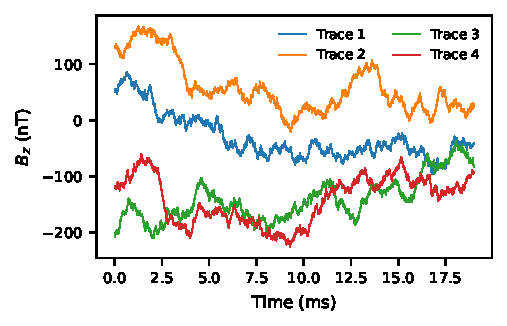
\includegraphics[width=\columnwidth]{fig_traces.pdf}}
\caption{Four of the one hundred recorded traces of effective magnetic field
noise. The traces wander on millisecond timescales and carry substantial static
offsets, both signatures of a strongly low frequency weighted spectrum.}
\label{fig:traces}
\end{figure}

\subsection{Noise characterisation}

Representative traces are shown in Fig.~\ref{fig:traces}. The ensemble standard
deviation is $\sigma_B = 95.1$~nT with a residual mean offset of $2.5$~nT. The
traces are visibly correlated over their whole length and differ markedly in their
mean value, which is the hallmark of quasi static inhomogeneous broadening.

The estimated spectrum is shown in Fig.~\ref{fig:psd}. Both estimators give the
same spectral shape, an inverse square power law
$S_B(f) \propto f^{-2}$ spanning the entire accessible band from $52.6$~Hz, set by
the inverse record length, to the Nyquist frequency of $200$~kHz. No knee is
visible, so the Lorentzian form
\begin{equation}
S_B(f) = \frac{4\sigma_B^2\tau_c}{1+(2\pi f \tau_c)^2}
\label{eq:lorentzian}
\end{equation}
appropriate to Ornstein Uhlenbeck noise fits the data well but constrains only the
product $\sigma_B^2\tau_c$, that is the high frequency amplitude
$S_B f^2 = \sigma_B^2/\pi^2\tau_c$; the fit returns $\tau_c \approx 56$~ms with
$\sigma_B$ correspondingly inflated to $135$~nT. Only a lower bound
$\tau_c \gtrsim 19$~ms can honestly be quoted for the correlation time, and this is
of no consequence for the coherence predictions below, which probe timescales far
shorter than $\tau_c$ and therefore depend only on the well determined product.
The direct autocorrelation estimator lies a factor of about $1.7$ above the Welch
estimate; this is spectral leakage, since the implicit rectangular data window has
sidelobes falling as $f^{-2}$, parallel to the signal spectrum itself, so that
low frequency power leaks uniformly across the band. The Welch estimate, whose Hann
taper gives $f^{-3}$ sidelobes, is used for all quantitative work.

\begin{figure}[t]
\centerline{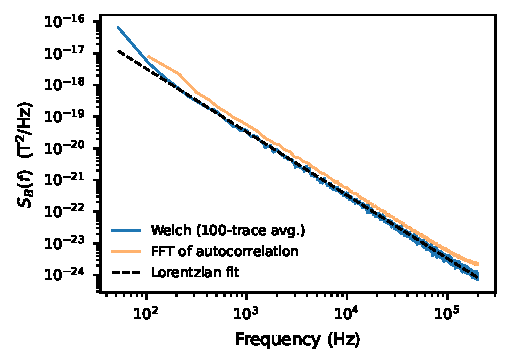
\includegraphics[width=\columnwidth]{fig_psd.pdf}}
\caption{Estimated one sided power spectral density of the field noise from Welch
periodogram averaging over the ensemble and from the Fourier transform of the
averaged autocorrelation function, with a Lorentzian fit. The spectrum follows
$f^{-2}$ over the whole band; the constant offset of the direct estimator is
window leakage, as discussed in the text.}
\label{fig:psd}
\end{figure}

\subsection{Coherence decay}

\begin{figure*}[t]
\centerline{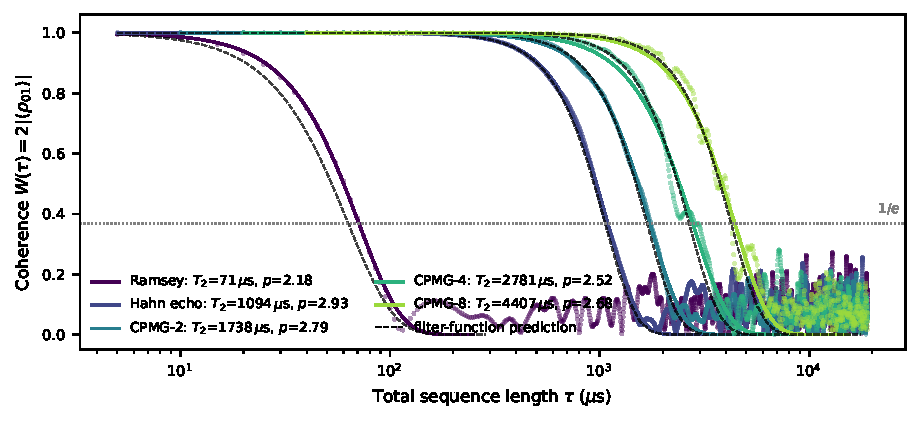
\includegraphics[width=\textwidth]{fig_decay.pdf}}
\caption{Simulated ensemble coherence against total sequence length for all five
sequences. Points are the trace based density matrix simulation, solid lines are
stretched exponential fits, and dashed black lines are parameter free predictions
from the measured spectrum via the filter function integral~\eqref{eq:chi}. The
scatter below $W \approx 0.1$ is the statistical floor of a one hundred spin
ensemble.}
\label{fig:decay}
\end{figure*}

\begin{table}[t]
\caption{Extracted Coherence Times and Fit Parameters}
\begin{center}
\begin{tabular}{lrrrr}
\hline
\textbf{Sequence} & \textbf{$N_\pi$} & \textbf{$T_2$ ($\mu$s)} & \textbf{$p$} & \textbf{$T_2^{\rm FF}$ ($\mu$s)}\\
\hline
Ramsey & 0 & $71 \pm 0$ & $2.18 \pm 0.02$ & 63\\
Hahn echo & 1 & $1094 \pm 1$ & $2.93 \pm 0.01$ & 1060\\
CPMG-2 & 2 & $1738 \pm 2$ & $2.79 \pm 0.01$ & 1680\\
CPMG-4 & 4 & $2781 \pm 15$ & $2.52 \pm 0.05$ & 2666\\
CPMG-8 & 8 & $4407 \pm 32$ & $2.68 \pm 0.08$ & 4235\\
\hline
\end{tabular}

\end{center}
\footnotesize $N_\pi$ is the number of refocusing pulses; $T_2$ and $p$ are from
the fit~\eqref{eq:fitfun} to the simulated decay; $T_2^{\rm FF}$ is the
parameter free prediction from the measured spectrum. Uncertainties are the fit
standard errors.
\label{tab:results}
\end{table}

Figure~\ref{fig:decay} shows the coherence decay for all five sequences and
Table~\ref{tab:results} collects the fitted parameters. The free induction decay
gives
\begin{equation}
T_2^{*} = 71.0 \pm 0.2\;\mu\mathrm{s}, \qquad p = 2.18 \pm 0.02 ,
\end{equation}
in good agreement with the quasi static prediction
$\sqrt{2}/\gamma\sigma_B = 84.5\;\mu$s from~\eqref{eq:quasistatic}; the residual
difference reflects the modest evolution of the field within $71\;\mu$s and the
finite ensemble. The exponent close to two confirms that the noise is essentially
frozen on this timescale.

A single refocusing pulse extends the coherence time by a factor of fifteen to
$1094\;\mu$s, with the exponent rising to $p = 2.93 \pm 0.01$. Additional pulses
give further gains, reaching $4407 \pm 32\;\mu$s for CPMG-8. The fitted exponents
for the decoupled sequences lie between $2.5$ and $2.9$.

\subsection{Comparison with the spectral prediction}

The dashed curves in Fig.~\ref{fig:decay} are computed from the fitted spectrum
through~\eqref{eq:chi} with no free parameters. They reproduce the simulated decays
throughout, and the coherence times agree to within four to ten percent across all
five sequences, as listed in Table~\ref{tab:results}. The agreement is the central
consistency check of this work: the spectrum estimated from the traces contains,
by itself, enough information to predict the outcome of the full density matrix
simulation.

\begin{figure}[t]
\centerline{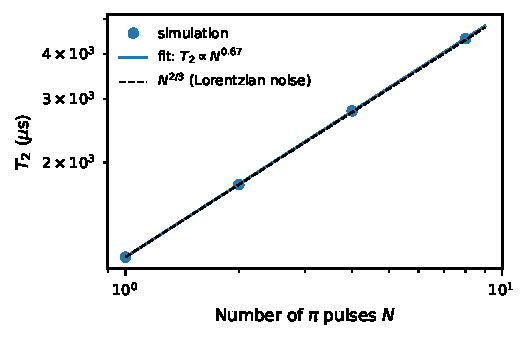
\includegraphics[width=\columnwidth]{fig_scaling.pdf}}
\caption{Scaling of the extracted coherence time with the number of refocusing
pulses. The fitted exponent of $0.67$ matches the two thirds law expected for
noise with a Lorentzian spectrum in the regime $\tau \ll \tau_c$.}
\label{fig:scaling}
\end{figure}

Figure~\ref{fig:scaling} shows the decoupling gain against pulse number. A power
law fit gives
\begin{equation}
T_2(N) \propto N^{0.67 \pm 0.02},
\end{equation}
indistinguishable from the exponent $2/3$ predicted for a spectrum falling as
$f^{-2}$ within the sequence passband.

\section{Discussion}\label{sec:discussion}

The results form a consistent picture in which a single spectral feature, the
$f^{-2}$ fall off, explains every observation.

The Ramsey decay is Gaussian because the spectrum is dominated by frequencies far
below $1/T_2^{*}$. In this quasi static regime each spin experiences an
essentially constant detuning drawn from a Gaussian of width $\sigma_B$, and the
ensemble average of $e^{-i\gamma B\tau}$ is the characteristic function of that
Gaussian, giving~\eqref{eq:quasistatic}. The measured $T_2^{*}$ of $71\;\mu$s
against the predicted $84.5\;\mu$s is agreement at the level one should expect
given that the quasi static formula neglects all dynamics.

The fifteenfold echo gain follows directly, since it is precisely the quasi static
component that the echo cancels. What survives is the noise evolving on the
timescale of the sequence itself, and for Lorentzian noise in the limit
$\tau \ll \tau_c$ the leading term is
$\chi(\tau) \propto \gamma^2 \sigma_B^2 \tau^3/\tau_c$, a cubic exponent. The
fitted $p = 2.93$ for the Hahn echo is a clean confirmation. The slight softening
towards $p \approx 2.5$ at larger $N$ is expected: the CPMG filter passband is
narrower and better approximates a single frequency, driving the decay back
towards the Gaussian form characteristic of a monochromatic filter.

The $N^{2/3}$ scaling has the same origin. With the filter passband centred near
$f \approx N/2\tau$ and the spectrum falling as $f^{-2}$, the decoherence integral
scales as $\chi \propto \tau^3/N^2$, and setting $\chi = 1$ gives
$T_2 \propto N^{2/3}$. The measured $0.67$ leaves little room for doubt. A
practical consequence is that decoupling here is a game of diminishing returns:
each doubling of the pulse number buys only a factor $2^{2/3} \approx 1.6$ in
coherence time, so the four hundredfold improvement from Ramsey to a
hypothetical thousand pulse sequence would demand pulse fidelities far beyond what
the ideal pulse assumption made here can justify.

Several limitations should be noted. All pulses are treated as instantaneous and
perfect, so no error accumulates with pulse number; in practice finite pulse
duration and rotation errors impose a ceiling on the achievable $N$, and CPMG is
chosen over Carr Purcell precisely because it is tolerant of such errors. The
ensemble of one hundred traces imposes a statistical floor of about $0.09$ in
coherence, restricting fits to the first decade of decay. The record length of
$19$~ms bounds the lowest resolvable frequency, so the correlation time is a lower
bound rather than a measurement, and the longest CPMG-8 coherence times approach a
non negligible fraction of the record. Finally, the model is one of pure dephasing:
transverse field components that would drive population relaxation are absent by
construction, so $T_1$ processes and the associated ceiling $T_2 \le 2T_1$ do not
appear.

\section{Conclusion}

An ensemble of one hundred measured magnetic field noise traces has been used to
simulate spin dephasing by direct density matrix propagation under explicit
rotation operators. The noise spectrum, estimated independently by Welch averaging
and by transformation of the autocorrelation function, follows an inverse square
power law across the accessible band. Free induction decay yields
$T_2^{*} = 71\;\mu$s with a Gaussian profile, a Hahn echo extends this to
$1.09$~ms, and CPMG with eight pulses reaches $4.41$~ms, the gain scaling as
$N^{2/3}$. Coherence times predicted from the measured spectrum through the filter
function formalism agree with the simulation to within ten percent without
adjustable parameters, demonstrating that the spectral characterisation and the
trajectory level simulation are two consistent views of the same physics.

\begin{thebibliography}{00}
\bibitem{b1} E. L. Hahn, ``Spin echoes,'' Phys. Rev., vol. 80, no. 4,
pp. 580--594, Nov. 1950.
\bibitem{b2} H. Y. Carr and E. M. Purcell, ``Effects of diffusion on free
precession in nuclear magnetic resonance experiments,'' Phys. Rev., vol. 94,
no. 3, pp. 630--638, May 1954.
\bibitem{b3} S. Meiboom and D. Gill, ``Modified spin-echo method for measuring
nuclear relaxation times,'' Rev. Sci. Instrum., vol. 29, no. 8, pp. 688--691,
Aug. 1958.
\bibitem{b4} N. F. Ramsey, ``A molecular beam resonance method with separated
oscillating fields,'' Phys. Rev., vol. 78, no. 6, pp. 695--699, Jun. 1950.
\bibitem{b5} G. Lindblad, ``On the generators of quantum dynamical semigroups,''
Commun. Math. Phys., vol. 48, no. 2, pp. 119--130, Jun. 1976.
\bibitem{b6} L. Cywinski, R. M. Lutchyn, C. P. Nave, and S. Das Sarma, ``How to
enhance dephasing time in superconducting qubits,'' Phys. Rev. B, vol. 77,
no. 17, p. 174509, May 2008.
\bibitem{b7} J. Bylander, S. Gustavsson, F. Yan, F. Yoshihara, K. Harrabi,
G. Fitch, D. G. Cory, Y. Nakamura, J. S. Tsai, and W. D. Oliver, ``Noise
spectroscopy through dynamical decoupling with a superconducting flux qubit,''
Nature Physics, vol. 7, no. 7, pp. 565--570, Jul. 2011.
\bibitem{b8} G. de Lange, Z. H. Wang, D. Riste, V. V. Dobrovitski, and
R. Hanson, ``Universal dynamical decoupling of a single solid-state spin from a
spin bath,'' Science, vol. 330, no. 6000, pp. 60--63, Oct. 2010.
\bibitem{b9} P. Welch, ``The use of fast Fourier transform for the estimation of
power spectra: A method based on time averaging over short, modified
periodograms,'' IEEE Trans. Audio Electroacoust., vol. 15, no. 2, pp. 70--73,
Jun. 1967.
\bibitem{b10} A. G. Kofman and G. Kurizki, ``Universal dynamical control of
quantum mechanical decay: Modulation of the coupling to the continuum,'' Phys.
Rev. Lett., vol. 87, no. 27, p. 270405, Dec. 2001.
\bibitem{b11} F. K. Malinowski, F. Martins, P. D. Nissen, E. Barnes,
L. Cywinski, M. S. Rudner, S. Fallahi, G. C. Gardner, M. J. Manfra,
C. M. Marcus, and F. Kuemmeth, ``Notch filtering the nuclear environment of a
spin qubit,'' Nature Nanotechnology, vol. 12, no. 1, pp. 16--20, Jan. 2017.
\bibitem{b12} J. Medford, L. Cywinski, C. Barthel, C. M. Marcus, M. P. Hanson,
and A. C. Gossard, ``Scaling of dynamical decoupling for spin qubits,'' Phys.
Rev. Lett., vol. 108, no. 8, p. 086802, Feb. 2012.
\end{thebibliography}

\end{document}
